% XeLaTeX can use any Mac OS X font. See the setromanfont command below.
% Input to XeLaTeX is full Unicode, so Unicode characters can be typed directly into the source.

% The next lines tell TeXShop to typeset with xelatex, and to open and save the source with Unicode encoding.

%!TEX TS-program = xelatex
%!TEX encoding = UTF-8 Unicode

%%  SPRINGER STUFF BELOW
\documentclass[graybox]{styles/svmult}

%%%%%%%%%%%%%%%%%%%%%%%%%%%%%%%%%%%%%%%%%%%%%%%%%%%%%%%%%%%%%%%%%%%%%%%%%%%%%%%%%%%%%%%%%
% Will Robertson's fontspec.sty can be used to simplify font choices.
% To experiment, open /Applications/Font Book to examine the fonts provided on Mac OS X,
% and change "Hoefler Text" to any of these choices.

\usepackage{fontspec}
%\defaultfontfeatures{Ligatures=NoCommon} 
%\setromanfont{Hoefler Text}
%\setsansfont[Scale=MatchLowercase]{Gill Sans}
%\setmonofont[Scale=MatchLowercase]{Andale Mono}

\usepackage[round]{natbib} % needed for Harvard style of references.
%\raggedright % To typeset the document with minimal hyphenation 
\usepackage[threshold=5,thresholdtype=words]{csquotes} % e.g. use smart quotes with a threshold level of 5 words before block indentation kicks in
\providecommand{\keywords}[1]{\textbf{\textit{Keywords ---}} #1}  % added to give basic keyword section
\usepackage{floatrow} % added to give better control over included images/figures
\usepackage[parfill]{parskip} % to typeset all paragraphs on new lines not indents.

%%  SPRINGER STUFF BELOW
\usepackage{mathptmx}       % selects Times Roman as basic font
\usepackage{helvet}         % selects Helvetica as sans-serif font
\usepackage{courier}        % selects Courier as typewriter font
\usepackage{graphicx}        % standard LaTeX graphics tool
\usepackage[bottom]{footmisc}% places footnotes at page bottom
%%  SPRINGER STUFF ABOVE


%%%%%%%%%%%%%%%%%%%%%%%%%%%%%%%%%%%%%%%%%%%%%%%%%%%%%%%%%%%%%%%%%%%%%%%%%%%%%%%%%%%%%%%%%

\title{The First (Beer) Living Lab: Learning to Sustain Network Collaboration for Digital Innovation}
%\title{Inter-Organisational Network Formation and Sense-Making: Initiation and Management of the Beer Living Lab}
\titlerunning{The First (Beer) Living Lab} % abbreviated version of your contribution title if the original one is too long
\author{Frank Frößler, Boriana Rukanova, Stefan Klein, Allen Higgins, Yao-Hua Tan and Séamas Kelly}
\authorrunning{Frößler et al.} 
\institute{Frank Frößler, Séamas Kelly and Allen Higgins (corresponding author), \at UCD School of Business, University College Dublin, Ireland, \email{allen.higgins@ucd.ie}
\and Boriana Rukanova and Yao-Hua Tan \at Department of Technology, Policy and Management, Delft University of Technology, Netherlands
\and Stefan Klein \at Institut für Wirtschaftsinformatik, University of Münster, Germany
}
%%%%%%%%%%%%%%%%%%%%%%%%%%%%%%%%%%%%%%%%%%%%%%%%%%%%%%%%%%%%%%%%%%%%%%%%%%%%%%%%%%%%%%%%%

\begin{document}
\maketitle

\abstract{
The Beer Living Lab was the first of a series of living labs established to analyse and improve complex cross-border trade and logistics challenges using innovative information technology. Unlike stable inter-firm networks where roles are formal and explicit, role taking and role assigning in the Beer Living Lab was highly dynamic. Although project deliverables were formally assigned, in practice responsibilities emerged as a result of actors' own initiative or as a result of negotiation and sense-making. Even leadership behaviour shifted throughout the various stages of the initiative. The practice of knowledge broking and cultivating a close working relationship with the operational manager emerged as crucial for creating and sustaining the social network which in turn stabilised the hybrid network organisation. We discover (yet again) the key practices of knowledge brokers and the necessity for social involvement in overcoming discontinuities within organisation networks.
}

\begin{keywords}
inter-organisational networks, sense making, network management, living-labs, knowledge broker
\end{keywords}

\section{Introduction}

There is a gap in our understanding of the social structures and collaboration processes that sustain Living Labs, even as they gain attention as real-life experimentation settings for developing and testing innovative technology. 
This study offers an in-depth analysis of the first living lab of the ITAIDE research and development programme\footnote{ITAIDE: Information Technology for Adoption and Intelligent Design for E-Government.}. 

The Beer Living Lab was designed as a platform for customs innovation\footnote{Earlier versions of this article were presented at the 20th Bled eMergence conference \citep{inter-orgNetworkFormation} and portions published \citep{rukanova2011beer, AcceleratingGlobalSupplyChains_ch14}}.
The problem addressed is the paradox of facilitating trade while maintaining control. 
Governmental, legal and regulatory environments all have a role in safeguarding the public good by controlling supply chains while at the same time facilitating economic activity. 
The on-going challenge for both business and government is how to innovate in regulated environments. 
Control of security, tariffs, excise and taxation raises the risk of duplicating or contradicting administrative, informational and technical needs. 
The need to enable transactions and traffic without losing control must accommodate the complexity of multi-stakeholder environments straddling these public and private domains. 

In the Beer Living Lab we found that the social, attitudinal, performative, linguistic processes were crucial to the initiation and management of a network of collaboration. 
Our analysis reveals the importance of negotiation, sense-making, and knowledge brokers. Living Labs demand subtle, complex social performances from their participants to produce the effect of an inter-organisational network.
The case highlights the importance of the practice of knowledge brokers and the varying activities which must be performed at different stages of the life cycle. It also makes a conceptual contribution by elaborating the concept of network practices on a social level, emphasising the importance of responding to contingencies of network collaboration over time. 


\subsection{What are Living Labs?}
\blockquote{A living lab is \enquote{a test environment for cyclical development and evaluation of complex, innovative concepts and technology, as part of a real-world, operational system, in which multiple stakeholders with different background and interests work together towards a common goal, as part of medium to long-term study}~\citep{lucassen2014living} }
Living labs were pioneered by William Mitchell at MIT's Media Lab and School of Architecture and City Planning~\citep{eriksson2006living} and have since been initiated in many different domains.
A living lab is a \enquote{naturalistic environment instrumented with sensing and observational technologies and used for experimental evaluation}~\citep{IntLarab}.
In particular, the approach mandates interventions -- building and experimenting with prototypes in live environments~\citep{AboAtkaa}.

The approach has been described as a \enquote{research methodology for sensing, prototyping, validating and refining complex solutions in multiple and evolving real-life contexts}~\citep{pierson2005configuring}. 
Positioned as real-life experimental settings for creating and evaluating new/changed technology, processes, and work practices; they suspend old rules to test new ones, to play with the possibilities of new social and organisational behaviours. 



\subsection{Living lab cases: social, spatial, temporal contexts}
Imperfect links between academia, policy, industry and societal sectors are blamed for innovation blocks \citep{burbridge2017if} for which Living labs are offered as a solution \citep{canzler2017living}. 
Unblocking the mutual flow of knowledge between university and business is the focus of urban living lab initiatives in Europe \citep{grotenhuis2017living, voytenko2016urban}. 

They have been used for whole-city trials of new technology applications; of electric vehicles in Málaga \citep{carillo2013smartcity}, for social geo-spatial mapping in Mexico \citep{sandoval2017open}, 

As systemic experiments in social innovation they have been used to conduct trials linking geographically and culturally distant sites between China and Finland ~\citep{tang2012internationally} 
They have been used to experiment with new modes of access and engagement between rural SMEs and central government in France, Greece, Latvia and Spain \cite{luccini2010egovtube}. 
Business and communities in Spain have been seeded with new technology incubators, to experiment with it in a purely exploratory fashion \citep{gasco2017living}. 

These examples explored novel combinations of technological apparatus (digital ecosystem), with technology in use (so called experiential computing) in an experimental social/spatial/temporal context \citep{nystrom2014actor}.
There is agreement that Living Labs refer to real-life, naturalistic settings for testing or evaluating concepts and/or technologies. 
They enable learning using in-the-wild settings as a bridge between the laboratory and the lived world; an open, uncontrolled yet \textit{focused} mode of public experimentation; (see table~\ref{tab:LL}). 

The duration of Living Labs may also be open-ended and stakeholders (e.g. technology providers, business and public organisations, users, and researchers) involved the whole time \citep{niitamo2006state}. 
Consequently, they activate an emergent attitude to design and innovation processes. 



\begin{table}[]
\centering
\caption{General characteristics of Living Labs research designs - (source:\cite[p. 129]{AcceleratingGlobalSupplyChains_ch14}}
\label{tab:LL}
\begin{tabular}{|p{0.4\linewidth}|p{0.6\linewidth}|}
\hline
Dimension            & Description                                                                                                                                                                                \\ \hline
Focus on innovation            & Acting to introduce novel social, organisational and technological objects.                                                                                                                \\ \hline
Broad setting                  & Comprise many people, organisations, locations, and extended duration.                                                                                                                     \\ \hline
Multiple methods employed      & Characterised as multidisciplinary research and development. Methods are disparate and ontologically distinct.                                                                             \\ \hline
Theoretical foundations varied & No one dominant theoretical foundation. Different domains may juxtapose but are not integrative. The contribution is to preserve theoretical complexity and distinctiveness of situations. \\ \hline
\end{tabular}
\end{table}



\subsection{Open innovation}
Not all problems addressed by technology are purely technical in nature, yet the political mind often misreads the power of technology. 
Even so, it is liberating to indulge in blue sky or magical thinking in order to address difficult problems. 
Echoing the idea of democratised innovation, a Living Laboratory mixes up the conventions of R\&D \citep{Hip2005aa}. Instead of pushing innovation, designs may be shaped by emerging demands \citep{pierson2005configuring}. Prototypes are adapted as users employ them in unexpected ways. Users and stakeholders become the source of innovation \citep{eriksson2006living,pierson2005configuring,henriksen2008pacta}.




Open innovation initiatives seek new ways of identifying value and value propositions around new arrangements of technology, product and service \citep{Ayvari:2017aa}. 
A focus on value implies attending to new ways of working, new hybrids of product/service, new user behaviours and emerging needs \citep{bjorgvinsson2012agonistic}.
They demand an intense focus on user involvement, on the co-creation of a good through the application of prototype arrangements to explore feasibility.


Living labs may also have a dark side. 
There is a tension between economic innovation and social innovation~\citep{vasin2017challenge}. 
So-called SmartCities initiatives~\citep{schaffers2011smart} have been accused of unrestrained data gathering from citizens in Dutch cities \citep{Naa2018aa}. 
Therefore, researchers need to ask; whose interests are served by these experiments in systemic innovation?
The aspiration for living labs is for \textit{all} stakeholders to be involved.
The systemic characteristics of living labs should enable actors to develop or uncover beneficial social innovation.
Social innovation in this sense occurs by \textit{involving} the public in collaborations that address social needs.





\subsection{Contributing to the living labs literature}
Much of the literature on Living Labs focuses on definition and justification, offering few insider accounts to aid and inform those involved in starting and running them \citep{budweg2011enhancing}. 
We seek to contribute to addressing this gap; to develop a better understanding of the practices, processes and social dynamics that support the initiation and subsequent management of Living Labs.
As \textit{development to research} initiatives we need better tools to understand how to successfully start them, how to galvanise actors, to achieve consensus, to enact and learn from \textit{collaborative innovation in the wild}. 


\section{Theoretical Framework}
What theories address an understanding of the origin of networks, of the situated, contingent local world in which people enact their organisations and networks, which they mesh together into bigger things? In a general sense, the term network is used to describe the structure of ties among actors in a social system \citep[p. 288]{nohria1994networks}. However, network studies tend to focus on the organisational or institutional level, offering little insight into how human actors initiate and enact to produce institutional and organisational structures. 
The following offers a practice theoretical view on the interplay between actors and institutional practices in order to better interpret the generative process of network collaboration.
 

\subsection{A practice theoretical perspective on network relationships}
A growing body of research on network relations recognises the complementary character of rational actor relations and relational theories. However, such work mainly concentrates on the macro-, inter-firm level \citep{schultze2004practice}. The problem with macro analysis is that it neglects the practice of individual members of organisations engaging in and managing boundary spanning activities at the micro level.
We adopt a structuration approach \citep{Gid1984aa} on the `practice theoretical' dynamics at work in the formation, production and reproduction of network relations (see \ref{fig:structuration}). 


% For figures use
%
\begin{figure}[b]
% Use the relevant command for your figure-insertion program
% to insert the figure file.
% For example, with the graphicx style use
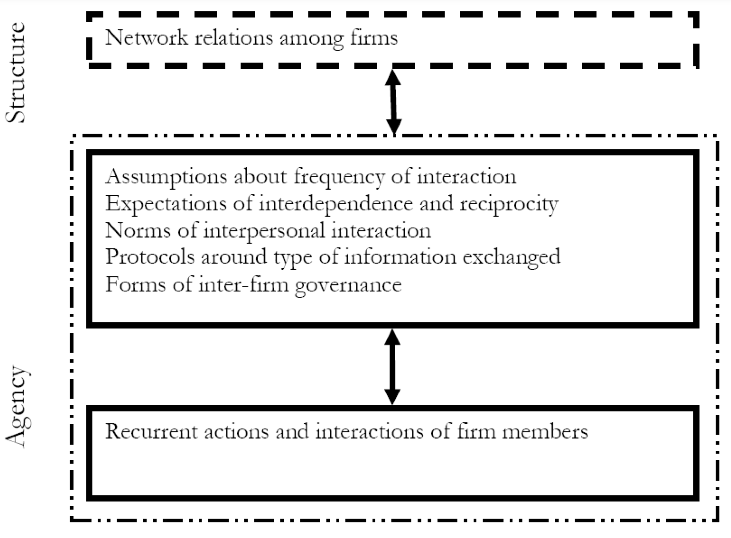
\includegraphics[width=\textwidth]{figs/structuration.png}
%
% If no graphics program available, insert a blank space i.e. use
%\picplace{5cm}{2cm} % Give the correct figure height and width in cm
%
\caption{Structuration view of networks (source: \citep[p. 89]{schultze2004practice})}
\label{fig:structuration}       % Give a unique label
\end{figure}


\subsubsection{Structuration}
Structuration argues that individuals enact social structure. The apparent force or structure of the social world comes about through recurring actions and interactions. Human actors employ their context, knowledge and assumptions to produce/reproduce social practices. The impression of social structure arises through repeated action; the performance of practices that enact ways of knowing the world. Organisations and power structures are constituted recursively through the expression of practices, for example: interactions, expectations of interdependency or reciprocity, norms of interpersonal relation, social protocols etc. They may extend to inter-organisational practices and in turn constitute wider social networks (considered to be network practices) - network structures performed by knowledgeable actors or agents \citep{SydWin1998aa}. Thus, actor/agents such as managers do not rely solely on institutional power or the structural properties of networks but also draw upon the rules and resources of extra-organisational resources, civil structure, governmental and society. Simply by enacting institutionalised practices the members constitute/re-constitute professional, organisational and inter-firm networks \citep{schultze2004practice}. 

A theoretical approach informed by structuration theory appreciates that it is individual members of organisations who enact boundary spanning practices and activity. The focus of researcher should shift therefore from abstract organisational entities to look more closely at the performance of individuals, their assumptions, norms, expectations, protocols and routines. 
Rather than limiting analysis to the inter-firm level, this approach attends to processual and contextual aspects encountered and performed by individuals along with their interpretive schemes,  beliefs, norms, and power relationships. As our theoretical foundation it offers a principled means of explicating contradictions, conflicts and the dynamics of network organisation and collaboration. 
In the following, we shall extend the practice theoretical perspective by referring to the communities of practice literature. We elaborate on sense-making processes within communities and the role of human agents in facilitating knowledge exchange across different communities.

\subsubsection{Communities and networks of practice}
Modes of knowing within a community are also ways of acting~ \citep{Wen1999aa}. Wenger uses the term negotiation to emphasise the productive process of meaning construction which is historical, dynamic, contextual and unique. 
Meaning is continuously negotiated over time as people experience the world and their engagement in it as meaningful. A community of practice engages constantly through the production and reproduction of shared meaning

Members from diverse organisations who engage in the same practices may perceive themselves as a network of practice; a shared identity arising from common, overlapping or similar practices \citep{brown2001knowledge}. Although the connections within a network of practice are less intense than those within a community, they do share commonalities allowing knowledge to circulate. In such networks diverse knowledge and practices may challenge each community's beliefs. 
Organisations, consisting of multiple communities of practices, can use their myriad of beliefs as the impetus for creativity and innovation, by tapping into and utilising the diverse practices of its own communities \citep{BroDug2000aa}. New communities may derive from a network of practice if they succeed in creating new sources of coherence, joint enterprise, mutual engagement, and shared repertoires \citep{Wen1999aa}.

\subsubsection{The knowledge broker}
Misunderstandings manifested during collaboration among different communities are balanced against actors' attempts to create coherence and bridge differences. 
Discontinuities, gaps or incoherence between different aspects of work may be evident in the form of temporal, spatial or organisational breakdowns \citep{beth2002discontinuities}. 
By clarifying mutual expectations, they may overcome misunderstandings and mitigate issues introduced by discontinuities. 

The pro-active engagement of human agents as knowledge brokers is positively related with attempts to bridge discontinuities between organisations and communities. Knowledge brokers help to generate shared tacit understanding among communities \citep{walsham2005knowledge} and increase awareness of other functional areas' working practices \citep{hayes2000work}. Brokers need sufficient knowledgeability of the practices, working cultures and discourses of each group if they are to phrase and reframe the interests of one community in a way which is meaningful to another \citep{BroDug2000aa}. Social legitimacy enables these agents to facilitate knowledge exchange and learning by way of linking and combining practices. Institutional practices such as boards, plenary sessions, formal meetings and the informal interactions that surround them are contexts for negotiating meaning among members from different communities. They offer the neutral ground in which participants produce mutual understanding and agreement \citep{Wen1999aa}. If enacted frequently these engagements become institutionalised and give rise to new knowledge and practices specific to the delegation and its participants. 


Based on this discussion a combined theoretical frame for analysing innovation in the BeerLL consists of the following. Structuration informs how action/interaction co-constitutes social structure. Practice theoretical perspectives offer ways of accounting for the performative dimensions of communities and networks. Communities of practice helps to understand the links between language and practice, the reifications of shared experiencing that occur all the time. 

\section{The Beer Living Lab}\label{sec:BLL}
The following case provides a detailed inside account of the social dynamics of the Beer Living Lab (Beer LL).
The analysis focuses on how its members generated shared understandings and galvanised action.

The Beer Living Lab was the first of a sequence of four living labs established under the ITAIDE  research project which ran from 2005 to 2010 as part of the EU 6th Framework for research and development~\citep{tan2006ecustoms}. 
These living labs created in-the-world environments for innovation experiments in areas impacted by government regulation and international standards. 

The Beer Living Lab focused on export/import logistics of excise\footnote{Excise duties are indirect taxes levied on licensed goods such as alcohol.} goods.
In the absence of tax harmonisation, the free movement of goods flowing through logistics networks and crossing borders within the EU creates difficulties for monitoring and controlling taxation.
Yet detailed monitoring and controlling adds administrative burdens adds costs to all involved.



\subsection{Research context}
Cross-border trade attracts the most demanding regulatory attention because of the value it produces and the risks it introduces \citep{henriksen2008pacta}. 
International trade must be monitored, reported and regulated or there is no control.
Yet consequent layers of administrative burden inevitably add cost to trade and degrade supply chain efficiency. 
The Beer Living Lab asked how new technology might help to overcome contradictions between the desire for `frictionless trade' against changing security and threat environments?

New technologies are seen to be key enablers. The Internet of Things (IoT), RFID, ubiquitous internet, GSM infrastructures, GPS telemetry, real-time monitoring; all offer the means to extend type and availability of trade information. These technologies promise the means to increase levels of supply chain control, efficiency and security. Administrative loads may be lessened by increased digital integration and information sharing between key actors in our trade supply chains, yet new forms of partnership or organisational relations may be needed in addition to new information technology.









\subsection{Research site}
The overarching goal of the Beer Living Lab was to demonstrate the feasibility of governments offering reduced administrative burdens to reliable companies, assuming they shared more data directly with authorities. 
It was assumed that trade simplifications could be built using new technologies -- Smart Locks, Internet of Things (IoT), GPS and GeoFencing -- while offering increased visibility, scrutiny, control and security on movements of goods between countries. 
The technological focal point of the BeerLL was a new kind of container seal technology coupled with new inter-organisational information systems (IOIS)\footnote{The Tamper-Resistant Embedded Controller (TREC) smart seal for container security developed by IBM, and a SOA, enabled by the Electronic Product Code Information Service (EPCIS) open standard from the global standardisation organisation GS1.}~\citep{rukanova2011beer}.

The Living Lab ran a series of live tests of whole systems for enhanced international trade.
It brought together a makeshift partnership of actors in order to experiment with new tools and new ways of enacting legally regulated activities.
The identities of partners and institutional stakeholders (figure~\ref{fig:consortium}) are listed below with abbreviations used for the case analysis:
\begin{enumerate}
\item BeerCo: Heineken N.V.
\item National Taxation and Customs Offices including: 
    \begin{itemize}
    \item DTCA - the Dutch Tax and Customs office
    \item TCA2 - HM Revenue \& Customs
    \item TCA3 - US Customs and Border Protection
    \end{itemize}
\item Researchers from National Universities including: 
    \begin{itemize}
    \item NU - Vrije University Amsterdam)
    \item NU2 - a joint team from University College Dublin and the University of Münster.
    \end{itemize}
\item  Technology, integration, consultancy and standards setting organisations:
    \begin{itemize}
    \item TechProv - IBM
    \item TechProv2 - comprised of GS1's EPCglobal, UN/CEFACT and the WCO.
    \end{itemize}
\item Sea Carrier - Safmarine, a subsidiary of the Maersk container shipping line.
\item 3PL subcontractors, telecommunications systems, GPS infrastructure and other stakeholders with indirect relationships to the network.
\end{enumerate}

% For figures use
%
\begin{figure}[b]
% Use the relevant command for your figure-insertion program
% to insert the figure file.
% For example, with the graphicx style use
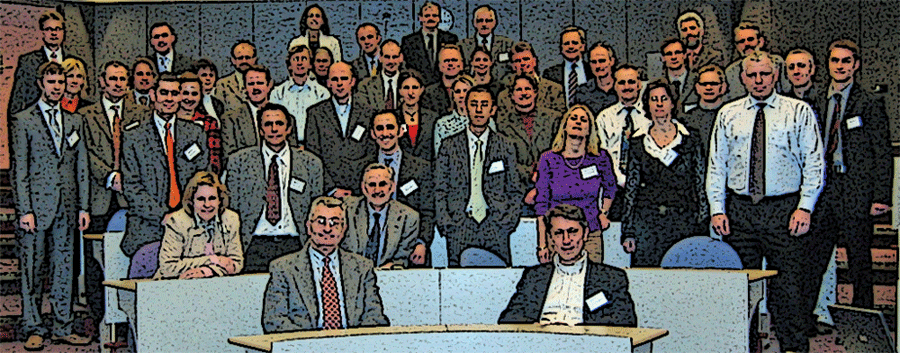
\includegraphics[width=\textwidth]{figs/ITAIDE_kick-off_group.png}
%
% If no graphics program available, insert a blank space i.e. use
%\picplace{5cm}{2cm} % Give the correct figure height and width in cm
%
\caption{ITAIDE consortium members at the kick-off meeting held at Vrije Universiteit Amsterdam (the Free University Amsterdam), March 1-3, 2006}
\label{fig:consortium}       % Give a unique label
\end{figure}

\subsection{Research Method}
\label{sec:method}
The case study follows the interpretative tradition \citep{Wal1995aa, Mye1997aa}. 
We employed a process approach~\citep{MarRob1988aa} which provides for a contextual analysis of the processes of change \citep{Pet1985aa}.
A narrative approach was used for the analysis and presentation of organisational processes \citep{pentland1999building}.
Guided by the theoretical/conceptual lenses of narrative and critical discourse analysis~\citep{boland1995perspective, phillips2012organizational}, we derived abstractions and generalisations, linking empirical details with abstract theoretical concepts. 
The analysis connected organisational \textit{structuring} with collaboration and individual actions, negotiation and sense-making. 

Data were gathered from different sources to build a comprehensive picture of the case including: 
\begin{enumerate}
\item Participation in workshops
\item Brainstorming sessions
\item Individual interviews with project participants
\item Participant observation
\item Document analysis
\end{enumerate}
University researchers (from NU, NU2 etc.) attended all general meetings, and many of the interactive sessions involving the partners. 
General project meetings and formal interviews were recorded and minuted. 
Findings from analyses were later reported on and presented to participants for validation and as a means of gathering further feedback.

Documentation analysed included EU and national policy documents, excise procedures, internal reports of TCA1, project reports etc.  
See table~\ref{tab:roles} for a summary list of the main interviewees (pseudonyms) their organisations and roles. Participant interviews lasting between 1 and 3 hours each were conducted throughout the project in order to continuously evaluate their perceptions and understandings.




\begin{table}[]
\caption{Interviewee pseudonyms and roles}
\label{tab:roles}
\begin{tabular}{p{0.2\linewidth}p{0.8\linewidth}}
\hline\noalign{\smallskip}
\textbf{Pseudonyms}	& \textbf{Interviewee roles}    \\
\noalign{\smallskip}\svhline\noalign{\smallskip}
Ron		& DTCA$^a$ process innovation group member and BeerLL coordinator \\ \noalign{\smallskip}
Joan	& DTCA customs auditor   \\ \noalign{\smallskip}
Steve	& DTCA client coordinator for BeerCo   \\ \noalign{\smallskip}
\hline \noalign{\smallskip}
James 	& BeerCo$^b$ customs manager and company liaison with DTCA    \\ \noalign{\smallskip}
Bob		& BeerCo internal tax auditor     \\ \noalign{\smallskip}
Jane	& BeerCo logistics manager   \\ \noalign{\smallskip}
\hline \noalign{\smallskip}
Rolf	& TechProv$^c$ technical coordinator for demonstrator development   \\ \noalign{\smallskip}
Frank	& TechProv customs subject matter expert \\ \noalign{\smallskip}
\hline \noalign{\smallskip}
Chris	& TechProv2$^d$ technical coordinator for interoperability and standards  \\ \noalign{\smallskip}
\hline \noalign{\smallskip}
Pat 		& NU$^e$ principal investigator and strategic project relationships  \\ \noalign{\smallskip}
John	& NU project manager  (operational, administrative)      \\ \noalign{\smallskip}
\hline \noalign{\smallskip}
Bobby	& UKTCA$^f$ Customs officer and liaison with DTCA and BeerCo \\ \noalign{\smallskip}
\hline \noalign{\smallskip}
Jack	& Sea Carrier$^g$ executive manager for applications \& services   \\ \noalign{\smallskip}
\noalign{\smallskip}\svhline\noalign{\smallskip}                                                            
\end{tabular}
$^a$ Dutch TCA -- Tax and Customs Administration of the Netherlands \\
$^b$ BeerCo -- international brewing Co.\\
$^c$ TechProv1 -- international computing services and hardware Co.\\
$^d$ TechProv2 -- international computing services \& hardware Co. \\
$^e$ NU-- national university \\
$^f$ UKTCA -- HM Revenue \& Customs \\
$^g$ Sea Carrier -- an international shipping Co.
\end{table}


\section{The Beer Living Lab: Case Analysis}

\subsection{Pre-project stage - creating a context}
The idea for the living lab research programme was triggered when Pat, a university professor at NU in the Netherlands, attended a conference.
Having previously prepared proposals but failing to obtain EU research funding, Pat had become acquainted with many officials in the various departments and agencies of the European Commission.
It was pointed out to Pat that a recent call for EU-funded research had been announced in his area of expertise. 
However, he knew from past experience that breadth and depth of academic and industry expertise was a prerequisite for a credible proposal, so he identified a small group of academic partners with whom he had long-standing relationships and who had an interest in contributing to the research proposal. 

They proposed adapting the Living Labs method in order to analyse complex cross-border trade and logistics challenges, and to respond by developing and studying the application of innovative information technology centred solutions.
Stakeholders composed of businesses, governmental agencies, universities and technology providers would come together to create, trial and explore more or less radical interventions in areas that had been resistant to change and innovation.

Four Living Labs were envisioned: experiments in administrative control of tax and tax-exempt trade; secure real-time transnational multi-modal cold-chains; data sharing among ecosystems of SMEs centred on a large manufacturer; and a unified food data model for pan-European trade.

Pat drove the first living lab, the BeerLL, in the Netherlands. 
First, he needed to involve a government agency, a company, and a technology provider.
Throughout his career Pat had worked as a kind of knowledge networker.
His personal interest in ideas around controlled borderless movements within the Customs Union attracted others in related organisations who believed in the potential for improvement, and his practice of making and maintaining professional connections embodied a nascent social network that was primed to crystallise around this project.

To gain interest from the government Pat got in touch with Ron whom he had known for more than 10 years. 
Ron had previously worked for the Customs department in Dutch TCA and had recently been given responsibilities for the \enquote{process improvement group} whose objective was to envision innovative IS solutions for the Dutch TCA. 

Ron reacted enthusiastically to Pat's suggestion to join the project because the BeerLL seemed to fit well with his new responsibilities. They discussed the latest policies and initiatives impacting Customs and Taxation and started working on a problem definition for the research proposal. 

Ron wanted the project to make an impact with a high volume of cross-border trade transactions. He had no direct customer contact, but he got in touch with a colleague (Steve), who was a client coordinator for a large beer producer (BeerCo) and was also responsible for leading an e-Business project within Dutch TCA. Steve became interested in contributing to Pat's research proposal as it was well aligned with his own e-business interests.

\blockquote{We were enthusiastic [about getting involved]\dots~on a higher level it looked like a new concept and we thought it is good also for the tax office to think about it. (Steve, Dutch TCA)}

Steve contacted the Customs Manager at BeerCo (James), however, it took another year before BeerCo would commit itself to joining the project.

\blockquote{BeerCo was not very enthusiastic at the beginning, they had to look at their costs, so they said, what's our benefit? So, we convinced them that benefit is a lot longer term. And they said, ok, we do it (Steve, Dutch TCA)}

To enrol a technology provider, Pat drew upon the existing institutional link between NU and TechProv and established a relationship with a board member of TechProv. At that time TechProv was conducting research and development into a new secure container seal technology with communication and sensor capabilities. TechProv was interested in setting up a pilot under realistic conditions and additionally saw an opportunity for strengthening the relationship with Dutch TCA as to learn more about e-Customs. 

Once Dutch TCA, BeerCo and TechProv became interested in the project, the universities began preliminary studies. 
The focused on revealing opportunities for improving cross-border trade. 
These interactions between NU, Dutch TCA, TechProv, and BeerCo were crucial for establishing an initial understanding of the problem area. 

\blockquote{They (TechProv and Dutch TCA) were the real motivation. I only had to align the interests and to coordinate the whole thing but at any moment in time I did not have to push anything. Because it was so much aligned with the strategic objectives\dots~And then the two managed to get BeerCo, not just involved, but to drive the process. (Pat, NU)}

With financial backing from TechProv and BeerCo, and part funding from the European Commission, contracts for the project were signed. 
The funding signalled credibility and gradually other organisations became interested, believing that Pat would make a success of the project. Selecting the right partners proved to be crucial for the later success of the network. The network found its origin in Pat's existing relationships but expanded wider due to his constant `networking', responding to serendipitous events, and producing action, all of which encouraged new players to become interested in the initiative. 


\subsection{Analysis and redesign stage}
Analysis and redesign yielded a new choreography for collaboration. In the pre-project stage, rather than being held together by shared interests, the network was merely a collection of stakeholders attempting to pursue their own self-interests. During the analysis and redesign stage, three key processes became essential for engaging the wider network of actors in the project and making the network work. These processes took place during general meetings and group interactions. They included 1) establishing initial social capital and shared understanding; 2) collaborating with others on specific tasks; 3) sense-making discussions integrating new learning and knowledge among groups. 

During general meetings, Pat and Ron acted as knowledge brokers in addition to their formal roles and were socially influential in the processes that took place. Pat's activities were focussed on mediation and translation between the network actors, who had different interests and different understandings of the problem domain. While in the initiation stage only a limited number of people were involved in setting up the project, when the BeerLL formally started, the organisations sent whole delegations of representatives. Sense-making processes needed to start again, now involving a larger group of people. These early general meetings were crucial opportunities for creating shared understandings, a shared language and shared purpose. This also held true for the later stages when redesigns were negotiated and where Pat again took a very active role in the negotiation of the revised solutions, making sure that the interests of all parties was considered. 

The following episode illustrates Pat's sense-making interactions. At this point BeerCo was still sceptical about the proposal from Dutch TCA about the redesign. Pat listened, interpreted, translated, and rephrased suggestions and tried to find acceptable solutions. 

\blockquote{
Pat: \enquote{So it would be a recommendation to EMCS\footnote{EMCS: Excise Movement and Control System. An EU customs system for monitoring the movement of excise goods.} from our point of view that they are able to cope with an AIN message \footnote{AIN message: Aangifte Informatie; digital trade declaration information.}. Basically, instead of imposing another message AIN is already in place and if the EMCS can be designed in such a way that it can take in an AIN message as input that will be a benefit for you?} \\
James: \enquote{Yes, of course.} \\
Pat:  \enquote{Your real advantage is that you don't have to build yet another system.} \\
James: \enquote{The real Single Window. That's really good.}
}
The accumulation of hundreds of these small interactions involving Pat and continuously cultivated by him and others within the network ensured that the BeerLL remained aligned with the multiple strategic objectives of the organisations involved. 

Ron too acted as a knowledge broker to stimulate innovation by gently questioning people's existing interpretations and re-framing problem areas. 

\blockquote{Ron is the key person when it comes to bringing innovation to the BeerLL\dots~ He was breaking taboos in the sense of questioning the traditional ways of working and assumptions underlying these ways of working (John, operational manager BeerLL, NU)}

\blockquote{ Ron has a long-term view. He is able to distance himself from the specific pilot and provide a long-term perspective, which compelled BeerCo to go along (Rolf, BeerLL Pilot coordinator, TechProv)}

With respect to the work groups that were formed, most of the time task allocation emerged naturally in the sense-making process in accordance with personal and institutional domain knowledge. While an overall resource plan for the project was sketched out, it was the responsibility of each organisation to make people and resources available on time for scheduled activities. This was not always an easy task as there were inherent differences in practices, such as perception of time and speed of work. 

\blockquote{For us this project was different than what we are used to. In this case [the BeerLL] sometimes we had to work fast to produce deliverables and sometimes we had to wait too long till the next phase. (Rolf, BeerLL Pilot coordinator, TechProv)}

John in his role as operational project manager took a slightly more instructive approach to coordinating efforts and facilitating the mutual adjustment of partners' understandings.

\blockquote{
John (remarked in retrospective): \enquote{It worked well;  when TechProv realised that it would work, but not the way they were used to.}
}
The analysis and redesign stages were marked by a gradual growing sense of community among the participants. They began to feel that they `were' of the BeerLL. They were developing their own jargon, terms and abbreviations borrowed from customs, logistics, manufacturing and technology. There was a growing sense that the project could make a difference, that the technology would influence the development of the next generation of systems. 


\subsection{The pilot and evaluation stage}
This period of the project might best be described as `Living Labbing in the wild'.
Shifting from the conceptual phase to the actual development of a pilot required further interaction and negotiation among the participants to decide on the scope of the pilot and the subset of information that was feasible to exchange in that setting. 
\blockquote{One of the main issues we encountered was to have BeerCo produce the correct files and help to interpret these files. This required close collaboration between TechProv and BeerCo (Rolf, BeerLL pilot coordinator, TechProv)}
After agreement was reached, TechProv, Dutch TCA and BeerCo had to line-up resources. TechProv had to ensure that the back-end systems and smart-seals used to monitor the shipment were operational. BeerCo had to ship containers with excise goods to the US and UK. Dutch TCA had to train personnel to perform inspections according to the new procedures. Dutch TCA had involve US and UK customs so as to guarantee that the necessary checks of the cargo were carried out in line with the new procedures. 

Everyone involved had to work closely together. Meetings were arranged to provide a holistic view of the pilot to build up a shared understanding of the pilot. Sessions were arranged to develop the training and procedures for those who would be working with the new system in the field. This new operational phase opened up new realms of uncertainty and risk required the participating organisations to re-engage in sense-making activities. 

Evaluation of the system started with another general technical meeting. The technical meeting was an opportunity to discuss issues that had occurred during the pilot, to identify areas for improvement, and even unexpected successes. This was followed by research interviews with the various stakeholders. 
The interviews gave people a chance to reflect on the process as well as make sense of the overall goals of the living lab. 

\blockquote{The process went very well. We were lucky to some extent; TechProv came at the right time with the innovative technology\dots~ for them the BeerLL was one of the first test sites of the smart seal. Dutch TCA needed a test case for AEO\footnote{AEO: Authorised Economic Operator - a licensed business status for operating in the international supply chain.} and SW\footnote{SW: Single Window for customs services.} and they wanted to try out these concepts; we (the university) provided fertile ground (Pat, Strategic Manager BeerLL, NU)}

\blockquote{When we started, my expectations were very low\dots~During the project things became clearer and I became more positive\dots~ I think that the ideas and the BeerLL concept are very nice and I am enthusiastic about them. If it depends on me, this is the future. I cannot be more positive than that! (James, Customs manager BeerCo NL) }
 
\blockquote{The change in mindset is the most valuable achievement from the BeerLL, the innovation lies in the major shift in thinking. (Joan, Customs auditor, Dutch TCA)}

The eventual outcome of the Living Lab was not considered to be `a finished product' or even the end result of a deliberately executed project plan. Instead a processual perspective helps us untangle complexity of happenings, interactions and produced relatively stable relationships in addition to a working system. These processes include; stabilising the network, initiating a cognitive shift towards a network strategy, and developing a supportive culture and practices (among others). 

The BeerLL began to be thought of as a platform for ongoing innovation among equal partners. 

\blockquote{In a Living Lab you as government are not in a position to exercise power. You need other mechanisms to drive people. Companies will do something only if the return on investment is clear. (Ron, BeerLL coordinator for Dutch TCA)}

Through their continuous engagement over time and against their historical and contextual backgrounds, the participants started to appreciate the fresh view the network offered. Understanding themselves as members of this network with its own unique identity brought about the sense of a joint enterprise with its own distinct understanding of the problem area. The process of generating common understanding was the precursor creating an innovative redesign scenario. 

\blockquote{Living Labs really require a lot from everybody\dots~if you have a relationship based on friendship, people will help each other; if they become very formal and calculate everything, then the whole thing will stop. In the BeerLL, all the partners made the extra mile to get the extra resources that were needed. (Pat, Strategic manager BeerLL)}

The project eventually fulfilled the objectives of the pilot and evaluation as the EU funding wound up. But the BeerLL did not cease to exist rather, its members moved to respond to the opportunities that had been revealed. 

\blockquote{The BeerLL provided a good starting point for discussions of how things could be done differently (Joan, Customs auditor, Dutch TCA)}

Even after the formal project concluded the actors continued to engage in sense-making processes, taking the lessons learned from the BeerLL to the next level, in pursuit of new goals. For Dutch TCA, the proof-of-concept from the BeerLL provided instruments to engage in political process of institutional change. Although the BeerLL as a time-bound project was over, its impact persisted through follow-on initiatives. 


\section{Findings and Discussion}
\subsection{The BeerLL as a Network}
The BeerLL falls under the broad definition of network as a \enquote{structure of ties among actors in a social system}~\citep{nohria1994networks}. However, it was distinct from an inter-firm network, such as strategic or R\&D alliances, as it involved a heterogeneous set of actors from different domains, notably the private and the public sector, which did not share a common goal (as is the case in strategic alliances or value-added partnerships) nor did they form a formal partnership as such. Rather, the BeerLL was an instance of a much broader political agenda and innovation initiative involving many organisations and institutions. 

It was difficult to draw clear boundaries around the BeerLL. For example, the Dutch TCA involved other national customs and tax administrations in the live technology demonstrator. Consequently, more emphasis was needed in the early phases of setting-up the network in terms of developing a joint agenda (sense-making and negotiation) as well as designing the joint activities. Given the experimental nature of the joint activities, processes of reflexive monitoring needed to be established to facilitate learning leading to adjustments to the structure and goal of the joint activities. 

While the BeerLL matched features of Living Labs more generally, it lacked the stability of a pre-existing social structure (e.g. an organisation, community, town, or city). 
Yet the openness of its scope was useful as it provided space for unexpected opportunities and areas for innovation. 
It offered a temporal conceptual space for a diverse collection of actors to attempt to reimagine their network of relations in response to digital innovation. 

\subsection{The BeerLL as Network Collaboration}
As a network of collaboration involving of players with different goals within a broader problem field, the BeerLL actually benefitted from having goals that were not all clearly defined. Yet while ambiguity and openness gave flexibility, it also complicated gaining commitment from participants. Even the end result, the technology proof-of-concept and live deployment, was only an intermediary product in pursuit of these further goals. As much as the outcomes remained quite open. It was difficult to steer the process and measure the outcomes. Thus, in the BeerLL we were confronted with moving targets concerning the clarity of goals, actors and results.

Key issues in the early stages were how to select partners and how to negotiate their involvement. 
Later, consensus forming among the participants was the challenge. The participants eventually agreed to more ambitious goals to run a whole-system proof-of-concept study under real world conditions. Yet the parties involved did not regard their relationship wholly as a 'partnership' as each pursued different goals, although all related to cross-border trade and logistics challenges.


\subsection{Coalition building as a prerequisite for collective action}

In a dynamic, open-ended environment, individual actors became active participants in enrolling new actors into the BeerLL. The initial legitimacy of the project was used to establish further, deeper involvement. They extended the technology capability with Geo-Fencing and real-time tracking and expanded the actor network by involving other TCAs and logistics suppliers. For these actors, social capital was critical to drive the negotiations and motivate a wide heterogeneous group of actors to provide resources and commitment to the joint activities. This reinforced our  finding that key actors captured the interests of others through direct personal involvement and commitment. Individuals enact negotiation and sense-making, but they interpret it in terms of their institutional and organisational contexts.

Rather than developing collaborative relationships, the BeerLL aimed at exploring common ground for collective action under the conditions of mutual dependencies of stakeholders who operate in separate domains. These actors normally enact rather antagonistic relationships characterised by mutual suspicion rather than trust. Yet within the shared environment of the Living Lab they were empowered to explore new ways of achieving radically different ways of relating with each other. This had benefits for private and public-sector actors through new ways of mutual coordination; new action, activities and knowledge. The BeerLL was like a loose coalition, where the partners found a consensus (for the common good), even if it involved compromising some of their own interests.


\subsection{A lifecycle perspective}
Although the BeerLL was an experimental setting rather than a full-scale implementation, it was at the same time a real-world project in which real resources were spent to make it happen. We regard three aspects as crucial for the actual initiation of the BeerLL. 

First, people and organisations enrolled in the network because they had formed an expectation that something would happen. This was based on Pat's networking, his boundary spanning and professional contacts. It was justified eventually by successfully gaining EU sponsorship for the research proposal. The consortium produced a perception of credibility and gave a signal that the initiative had high level institutional commitment. 

Second, the funding that the EU provided turned out to be critical as it helped to initiate joint activities with others beyond the consortium. Modest financial supports allowed peripheral and central actors to meet and discuss how to engage in collective action. Support for travel and meetings enabled participants within all organisations a degree of budgetary independence from the constraints of their own organisations. Eventually, many invested additional resources to participate and learn from the living lab. 

A third element which we found crucial for the initiation of the BeerLL was the behaviour of key people spontaneously acting as knowledge brokers. These knowledge brokers were also local initiators, the people who took the initiative, came-up with ideas and started the process of engaging with others, of linking organisations.




\subsection{Network activities and practices}
Initially the BeerLL was a fragile social/institutional network which could in principle have broken-down at any stage. We recognised how crucial the behaviour of knowledge brokering is to network collaboration. Pat and John kept the network together during the whole process through their involvement in overcoming discontinuities within the network \citep{beth2002discontinuities}. 
Importantly, knowledge broking is seen in dyadic, triadic and group collaboration performances. For example, Pat and Ron, acted as complementary knowledge brokers and carried out different activities throughout the whole process. 
In another example, John, the operational manager, Rolf in TechProv and Steve in DTCA came together as a kind of communications back-channel that helped to keep the network together. 
Pat, through his activities of initiation, mediation and translation, became instrumental in the negotiation and sense-making processes for everyone and this was crucial for keeping the fragile network together. Pat could assume and maintain this role as he had the status to do that (being a professor, as well the research project coordinator).
He was politically sensitive and neutral, constantly searching for the common denominator. These characteristics enabled the others to accept him in his role as a knowledge broker. 
Ron too was active in sense-making and sharing knowledge among wider groups. In the early stages of the project he was fundamental in framing the initial problem of the BeerLL as he had a very in-depth knowledge of the domain. In the analysis and redesign phase, he focussed on innovation facilitation. 



\subsection{Tolerance towards ambiguity an open-ended dynamic}
In traditional networks, there is usually an expectation that the network will stabilise for a period and function steadily if maintained \citep{Riemer2006}. This was not the case in the BeerLL which was open-ended and dynamic. Nor was it the goal of the BeerLL to achieve a long-term stable state of operation for continuous activities. Its goal was short-term, to simply test proofs-of-concept. The prototypes needed only operate a short time. They changed, were tweaked and did not need to be sustained indefinitely. As each learning experience was discussed and made sense of, the network proceeded to undertake some new change. The social network embodied new learning leading to new goals e.g. recommending necessary changes to legislation or altering technology capability. The experimental character of the Living Lab was a strength because it allowed for trial and error. Failures became an inevitable part of the learning rather than something to be avoided.


\section{Concluding remarks}
Previous research into Living Labs has concentrated on the objectives of these enterprises while neglecting to reveal the underlying social processes of their formation and management. 
Our research reveals the Living Labs to be a social network of collaboration and of practice. 
Participants must be therefore become sensitive to the interactive and social dynamics of a Living Lab setting. 

By definition Living Labs lack well defined boundaries or predictive goals. They demand continuous sense-making and negotiation. 
They are fragile states of engagement and remain fragile throughout their life cycle. The success of a Living Lab is never secured, it is instead the result of continuous effort, of engaging in sense-making and knowledge broking activities.  
While a single case is insufficient for generalisation, this extensive study offers empirical evidence and contributes to a growing body of research shedding light on the social performances involved in and needed to sustain Living Labs and network collaborations more generally.


 % Springer referencing style, in this case spbasic 
\bibliographystyle{styles/spbasic}
%\bibliographystyle{apalike}% or plainnat or apalike or agsm (both Harvard style kinds)
 \bibliography{bibtex/referenc_01}

\end{document}